\section{Semantic Web}
The term \emph{``Semantic Web''} was first introduced by Tim Berners-Lee in 2001\cite{berners2001semantic}. The Semantic Web was established to solve the main problem of the Web, being that the Web is readable for humans, but not for machines. With the Semantic Web, machines should be able to interpret the Web. These machines are called intelligent agents and they will be able to fulfill complex tasks autonomously.\\

\noindent To achieve this goal, a preliminary step is that publishers of data must be able to assign a meaning to the elements of the dataset. More specifically, machines must be able to understand this meaning without human intervention. Since datasets can have a variety of natures and topics, there is a need for so-called \emph{ontologies}, which can be compared to vocabularies for humans. However, vocabularies define terms and ontologies define how these terms are related, mostly for reasoning. Finally, the Semantic Web must be \emph{decentralized}, which means that data should not be contained on a single or a few servers\cite{berners2001semantic}.

\subsection{Semantic Web Stack}
The architecture of the Semantic Web is based on a hierarchy of technologies. This hierarchy is composed as a bottom-up approach, in which every layer uses the layer(s) directly beneath to achieve its goal. This strategy is visualized in \Cref{fig:semanticstack}. Since the subject of this paper is the publishing of data, only the layers that are relevant to this extent are considered. In the figure, this corresponds to the bottom five layers (indicated in bold).

\begin{figure}[t!]
    \centering
    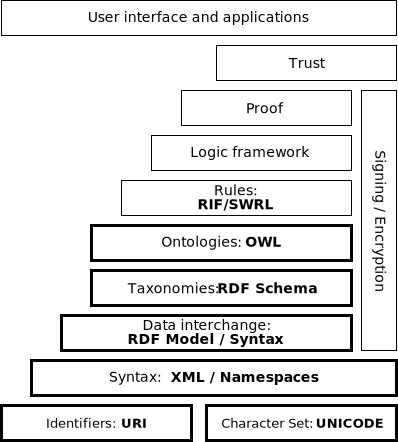
\includegraphics[width=0.9\textwidth]{images/semantic-web-stack.pdf}
    \caption{Semantic Web Stack (based on \cite{semanticwebstack,semanticwebstack-wiki}). This image reflects the original Semantic Web Stack from 2001. As a result, some of the technologies are outdated or deprecated (e.g. URI and XML). The relevant technologies for this paper are indicated in bold.}
    \label{fig:semanticstack}
\end{figure}

% Required to fix widow sentence.
\newpage

\subsubsection{Unicode}
Unicode\footnote{\url{https://unicode.org/standard/standard.html}} is a system that is used to guarantee a consistent encoding, representation, and handling of text. Similar to ASCII, Unicode was established to aid developers in the creation of applications. However, the advantage of Unicode is that it solves the problems that exist in previous encoding schemes, such as the inability to encode all characters. This problem in particular is tackled by assigning an identifier to each character on every platform, for every program, and in every language.

\subsubsection{Uniform Resource Identifier (URI)}
A URI offers a uniform way to identify an object. This identifier is often confused with a \emph{Uniform Resource Locator (URL)}, which \emph{locates} an object, rather than \emph{identifying} it. Consequently, every URL is an example of a URI, but not vice versa\footnote{\url{https://www.w3.org/Addressing/URL/uri-spec.html}}.

\noindent Together with Unicode, which was a W3C recommendation for the Web, URI resides at the foundations of the Semantic Web Stack. This combination enables the identification of resources on the Web uniformly.

\subsubsection{Extensible Markup Language (XML)}
XML is used to describe data. The most important traits of XML are that it is a flexible, simple and extensible format to store data. XML defines elements using so-called ``tags'', with every element having both a start-tag and an end-tag. Furthermore, XML supports nested elements, enabling the creation of hierarchies. Since it was a W3C recommendation, XML is at the lower part of the Semantic Web Stack.

\subsubsection{Resource Description Framework (RDF) Model, Syntax and Schema}
The final element of the Semantic Web Stack is RDF, which is used to add meta-information to a dataset in a describing way. Due to the importance of RDF for the rest of this paper, it is explained in detail in \cref{ssec:formatting-RDF}.